\subsection{Pivot and Travel Limiter}
\subsubsection{Description}
The main function of the pivot was to reduce the bending that would be transmitted to the output drive shaft from the drive box and protected the shaft from debris or other objects. Another function of the pivot was to limit the rotation of the exterior drive box to a certain range of rotation. Limiting the rotation was a bumper component fastened with ten 5/16" bolts to the end of the pivot and located on the interior of the chassis. This limiter only allowed a rotation of $\pm$30\degree. The pivot was designed to have interference fits for housing mounted seals and the outer races of taper roller bearings. Figure~\ref{fig:pivot_assembly_drw} shows the final design of the pivot assembly and Figure~\ref{fig:pivot_bld} shows the manufactured pivot.
\begin{figure}[H]
\centering
\begin{minipage}{0.45\linewidth}
\centering
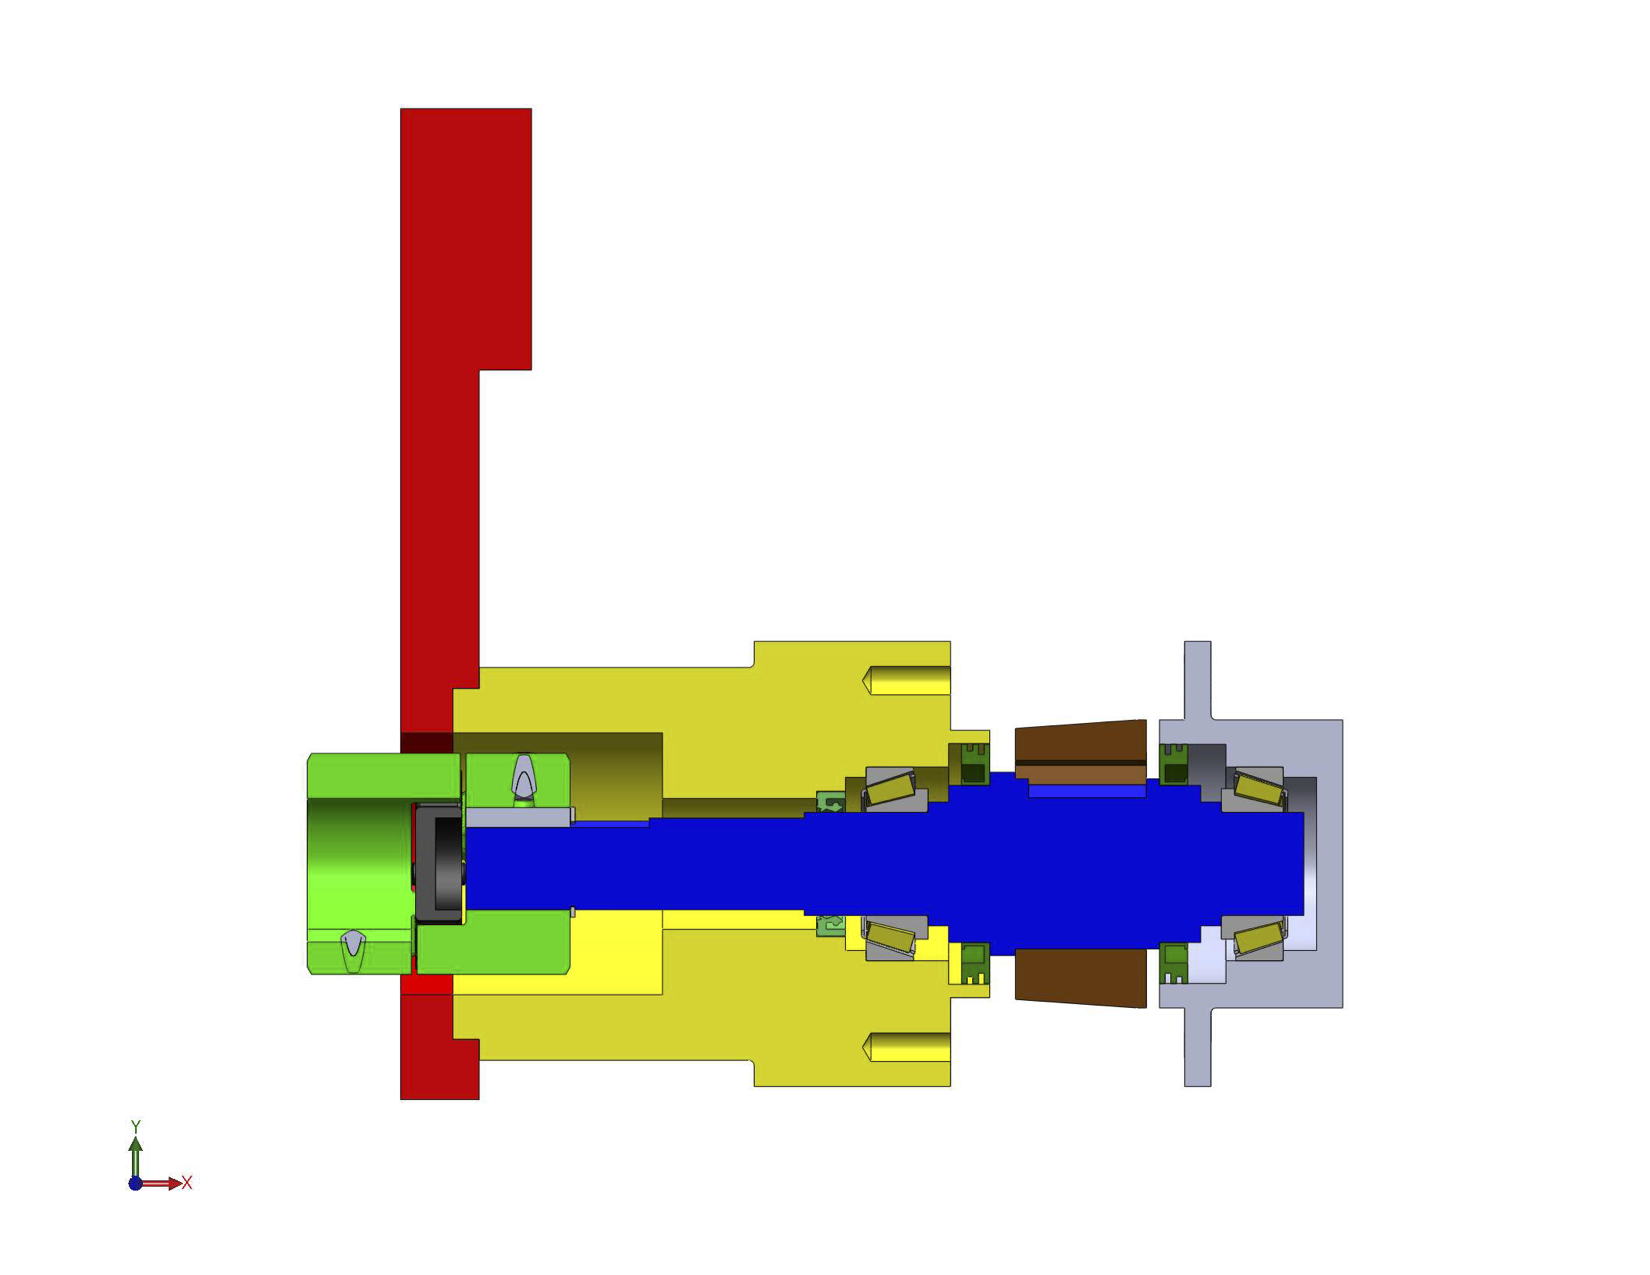
\includegraphics[width=0.9\linewidth]{./images/pivot_assembly_drw}
\captionof{figure}{The pivot is shown in yellow and the limiter is shown in red}
\label{fig:pivot_assembly_drw}
\end{minipage}
\begin{minipage}{0.45\linewidth}
\centering
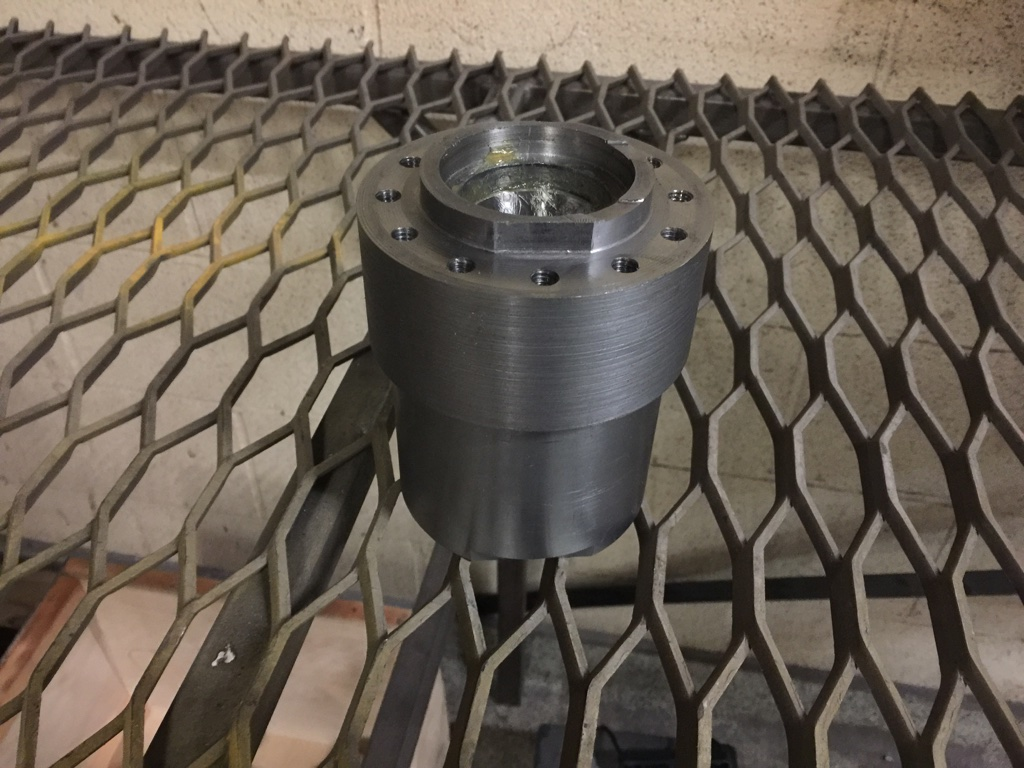
\includegraphics[width=0.9\linewidth]{./images/pivot_bld}
\captionof{figure}{Manufactured pivot.}
\label{fig:pivot_bld}
\end{minipage}
\end{figure}

\subsubsection{Design Constraints and Functional Requirements}
The design of the pivot was dimensionally constrained in both its allowable inside and outside diameters as well as the required overhang of the flanged section from the vehicle body. The diameter of the flanged section would also need to be able to accommodate a sufficient number of appropriately sized fasteners for attachment to the drive box, and be sufficiently larger than the pivot body diameter to keep the pivot section axially located against bushings pressed inside the pivot mounting hole in the frame of the vehicle. Additionally, the travel limiter was constrained by the required range of rotation for the pivot, with the travel limiter having flat contact surfaces on both sides. Furthermore, it was necessary for the pivot to remain attached to gear box during assembly and disassembly, with the placement of the pivot to be axially located using two opposing flanges on each of the pivot section and travel limiter. This design would necessitate a simple method of attaching the pivot to the travel limiter to allow for ease of assembly of the drive box to the frame. Table~\ref{tab:pivot_const} outlines the design constraints of the pivot. Finally, the pivot needed to incorporate shoulders to accommodate press fitting the outer race of taper roller bearings and shaft seals inside.
\begin{table}[H]
 \centering
 \caption{Pivot Design Constraints and Requirements}
 \begin{tabular}{| p{4cm}lp{2cm}p{7cm} |} \hline 
 Constraint & Value & Unit & Reasoning \\ \hline
 Max OD & 4 & inch & Constrained by dimensions of frame section available for support \\
 Min ID & 2 \textsuperscript{1}/\textsubscript{4} & inch & Chosen to accommodate a coupling to attach drive shaft to driven, output shaft, with a \textsuperscript{1}/\textsubscript{8}'' space between the coupling and the inner wall of the pivot \\
 Pivot section outside the vehicle & 1 & inch & To provide spacing between the drive box and the outer frame of the buggy and to accommodate fasteners for drive box attachment \\
 Flange diameter for both pivot and travel limiter & \textsuperscript{1}/\textsubscript{4} & inch & Provide contact surface between flanged face and bushing face. Axial location of pivot within frame mounting section. Bear axial loads applied to pivot during skid steer operation \\
 Angular travel limit for pivot and limiter assembly & 60 & degrees (full range) & Angular range of rotational motion of entire gearbox assembly to prevent contact with upper compartments of frame assembly \\
 Ease of assembly & - & - & General constraint which specifies the need for the pivot section to be attached to the travel limiter, as a two piece assembly, allowing for quick assembly and removal of the gear box \\ \hline
 \end{tabular}
 \label{tab:pivot_const}
 \end{table}

The purpose of the pivot was to house the drive shaft as well as support the weight of the buggy while connecting the drive box to the rest of the vehicle. It was designed to be modular, and considerations were taken to minimize pinch points during assembly, disassembly and maintenance. The travel limiter formed the back half of the pivot assembly and sat inside the vehicle body. Its purpose was to limit drivebox rotation to $\pm$ 30\degree. Stopping the rocker arm of the travel limiter were two rubber stoppers fastened to the modified frame section on the interior of the buggy. The implementation of the rubber stoppers was to prevent deformation of frame members and reduce the effects of the impact from the stopper arm, however since the angular rotation of the driveboxes were assumed to travel at 3.6\,rpm, the impacts would be relatively minor and static loading conditions were investigated.  

\subsubsection{Alternate Solution}
A few alternative solutions for the pivot were investigated before a final design was specified. Each design was an iteration of the previous, with modifications made to accommodate the addition of bearings and seals, as well as the accommodation of a removable shaft coupling in more recent iterations. Finite element analysis was performed to determine overall strength of the pivot and was used to reduce the size of the travel limiter.

Figure~\ref{fig:pivotold} and Figure~\ref{fig:pivotfinal} illustrate the intermediate design of both the travel limiter and the final pivot design. It can be seen from the old design that the travel limiter underwent design change where the final design is less complicated to make and was overall a more efficient solution. This version of the design was made with shoulders for a press fit taper roller bearing as well as two shaft seals. The previous iteration of the pivot design saw increases in outer diameter to nearly 4 1/2 ", which was increased to incorporate the addition of taper roller bearings. Again this design was meant to provide shoulders for both shaft seals and bearings, and be able to provide clearance for the drive shaft. Figure and Figure ,illustrate the second design concept. It can be seen that this design made use of twelve 5/16"- 24 bolts to secure the pivot to the drive box. A further ten bolts of the same size were used to fasten the travel limiter to the pivot. The flange diameters for both the travel limiter and the pivot are equal in this design.

\begin{figure}[H]
\centering
\begin{minipage}{0.45\linewidth}
\centering
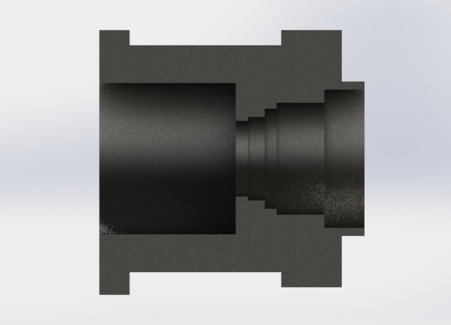
\includegraphics[width=\linewidth]{./images/oldpivothaft}
\captionof{figure}{Original pivot design}
\label{fig:pivotold}
\end{minipage}
\begin{minipage}{0.45\linewidth}
\centering
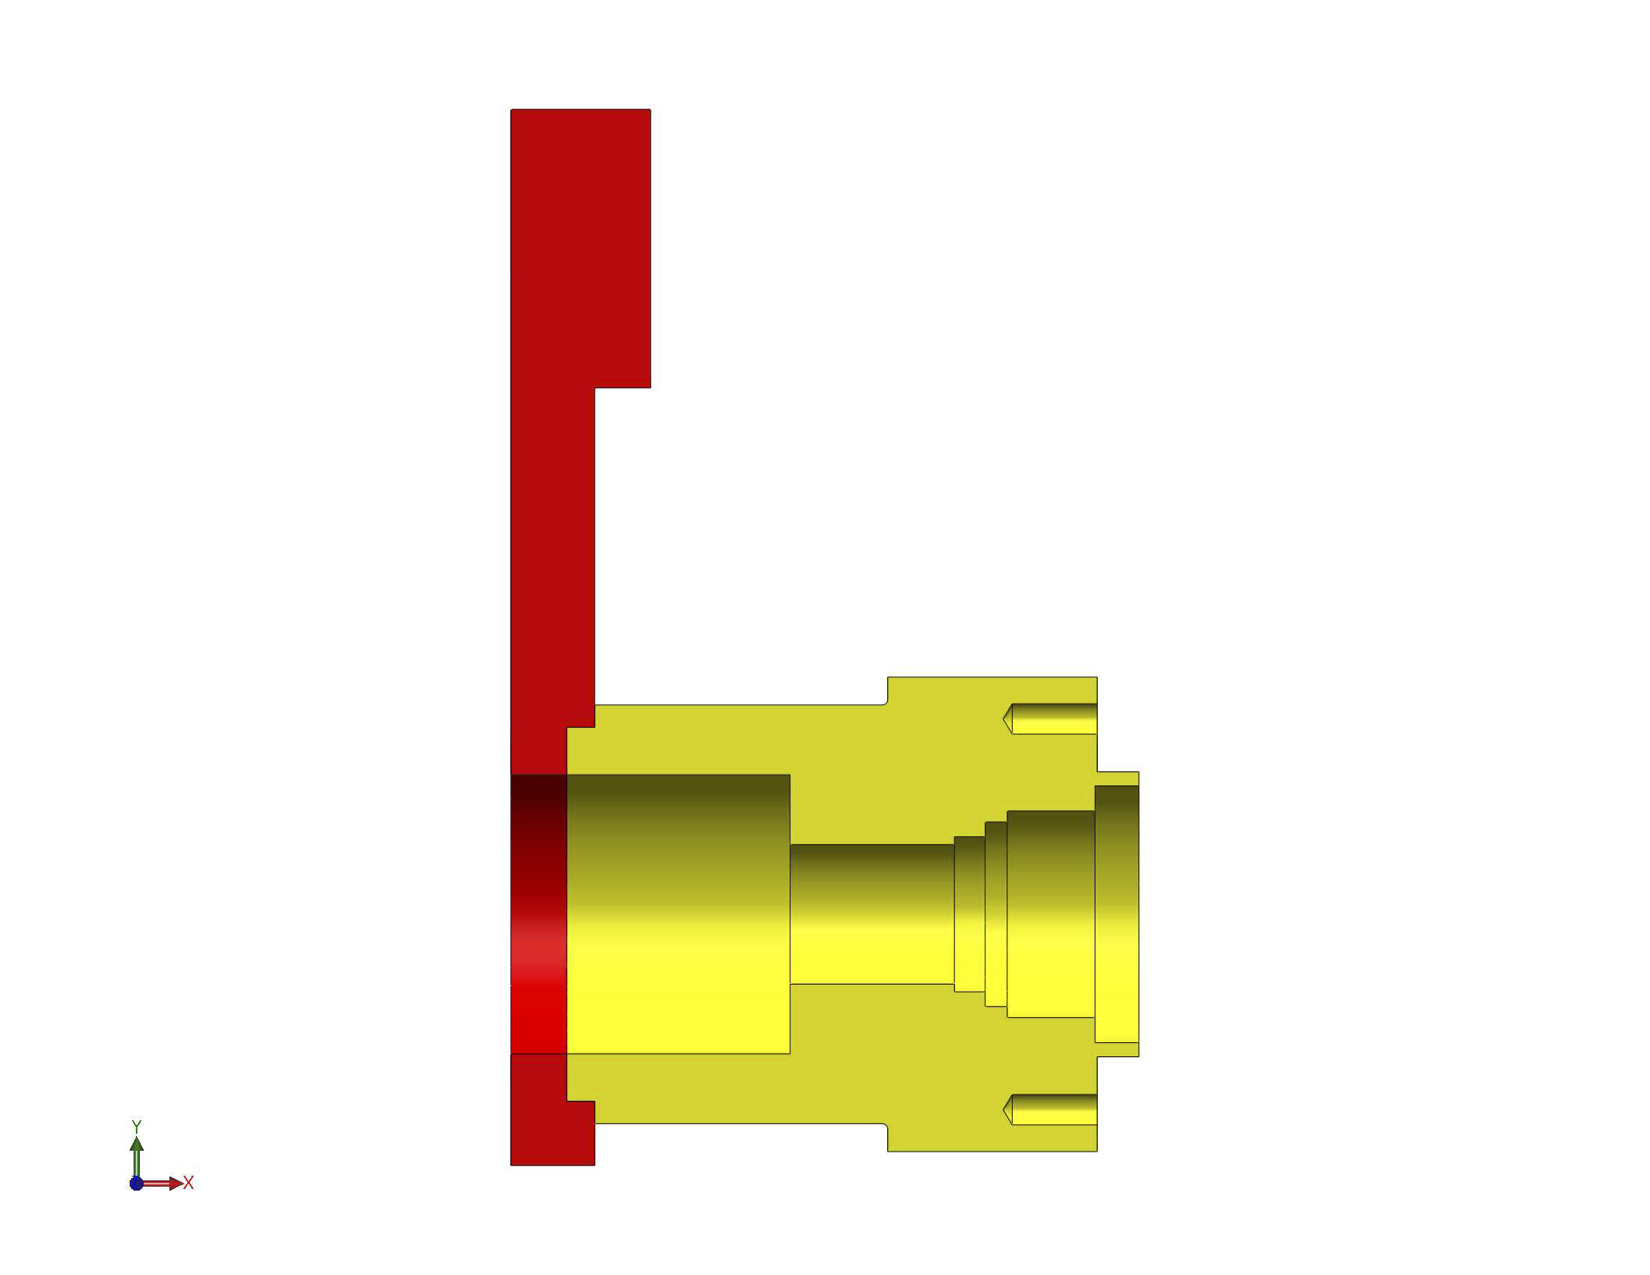
\includegraphics[width=\linewidth]{./images/finalpivot}
\captionof{figure}{Final pivot design}
\label{fig:pivotfinal}
\end{minipage}
\end{figure}

In the final version of the pivot the length of the pivot body was increased by 1/8'', while the part of the pivot sitting outside the vehicle was reduced by 1/8''. Additionally, the final pivot design had two fewer bolt holes than the original design to prevent overlapping of countersunk holes in the drive box back plate. Finally, the rocker arm of the travel limiter was changed to be oriented vertically upward as opposed to its previous vertical downward orientation.

\subsubsection{Analysis and Design}
The pivot and travel limiter design went through four iterations. Each iteration was improved using FEA tools in SolidWorks with the emphasis on increasing strength and reducing unnecessary material. In Appendix~\ref{sec:pivot_fea} the FEA can be found for each revision. Figures~\ref{fig:pivot_stress_fea}~and~\ref{fig:old_pivot_stress_fea} show a comparison between the first and final iterations.

The Von Mises stress maps show the stress concentrations around the pivot shoulder. A fillet was added to reduce the stress concentration in that area. Also the step down diameter was increased to fit the new seal for the taper roller bearing that is located in the pivot.


